\documentclass[12pt]{article}
\usepackage[fleqn]{amsmath}
\usepackage{graphicx} 

\begin{document}
\pagenumbering{Roman}
\title{Exploratory Models}
\author{Gregory Guranich}
\date{\today}
\maketitle
\tableofcontents
\hfill \break
\hfill \break
\\
\\

\newpage

\section{Notation}
\indent\textit{notation in rscript is not up to date}
\begin{description}
\item{satisfied contraceptive limiting = } cl
\item{satisfied contraceptive spacing = } cs
\item{unmet limiting = } ul
\item{unmet spacing = } us
\item{unmet = } ul + us
\item{total limiting = } cl + ul
\item{total space = } cs + us
\item{total demand = } cl + cs + ul + us
\item{limiting out of demand(PDL, formerly luup) = } $ \frac{cl + ul}{cl + cs + ul + us} $ = $ \frac{total Limiting}{total Demand} $
\item{limiting out of Unmet (LUP, formerly lup) = } $\frac{ul}{ul+us} $ = $ \frac{unmetLimiting}{unmet} $
\item{ratio of satisfied needs (ratio, formerly ratio) = } $\frac{\frac{cl}{cl+ul}}{\frac{cs}{cs+us}} $ = $\frac{\frac{satisfied Limiting}{total Limiting}}{\frac{satisfied Spacing}{total Spacing}} $ 
\item{}
\end{description}

\newpage

\section{PDL Varying Intercept Models And Slope(without shrinkage on slope)}
\pagenumbering{arabic}
$ y_i|\mu_{ct},\sigma_y \sim N(\mu_{ct}, \sigma_y) $ \\
$ logit(\mu_{ct})=  \pi_{ct} $\\
$ \pi_{ct} = \alpha_c + \beta_c*demand_{ct} $\\
\\
$ \beta_c \sim N(0,100) $ \\
$ \alpha_c|\alpha_r,\sigma_{c\alpha} \sim N(\alpha_r,\sigma_{c\alpha}) $ \\
$ \alpha_r|\alpha_w,\sigma_{r\alpha} \sim N(\alpha_w, \sigma_{r\alpha}) $\\
$ \alpha_w \sim N(0, 100) $\\

\noindent
 $ \sigma_y \sim U(0,2) $ \\
 $ \sigma_{c\alpha} \sim U(0,2) $ \\
 $ \sigma_{r\alpha}\sim U(0,2) $ \\
\\
\begin{center}
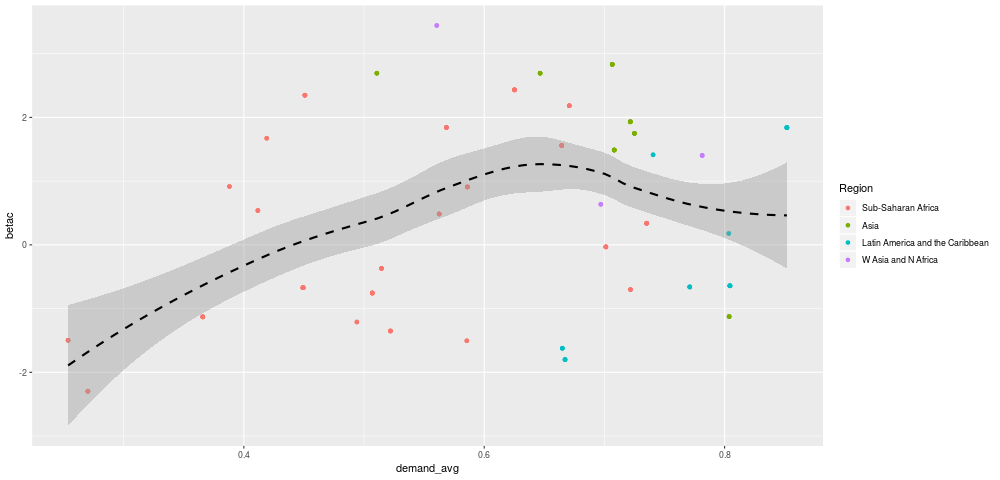
\includegraphics[scale=0.4]{1.png}
\end{center}
\newpage
\section{PDL Varying Intercept and Slope Models}
\subsection{without correlation}
$ y_i|\mu_{ct},\sigma_y \sim N(\mu_{ct}, \sigma_y) $ \\
$ logit(\mu_{ct})=  \pi_{ct} $\\
$ \pi_{ct} = \alpha_c + \beta_c*demand_{ct} $\\
\\
$ \beta_c |\beta_r,\sigma_{c\beta} \sim N(\beta_r,\sigma_{c\beta}) $ \\
$ \beta_r|\beta_w,\sigma_{r\beta} \sim N(\beta_w, \sigma_{r\beta}) $\\
$ \beta_w \sim N(0, 100) $\\
$ \alpha_c|\alpha_r,\sigma_{c\alpha} \sim N(\alpha_r,\sigma_{c\alpha}) $ \\
$ \alpha_r|\alpha_w,\sigma_{r\alpha} \sim N(\alpha_w, \sigma_{r\alpha}) $\\
$ \alpha_w \sim N(0, 100) $\\

\noindent
 $ \sigma_y \sim U(0,2) $ \\
 $ \sigma_{c\alpha} \sim U(0,2) $ \\
 $ \sigma_{r\alpha}\sim U(0,2) $ \\
\begin{center}
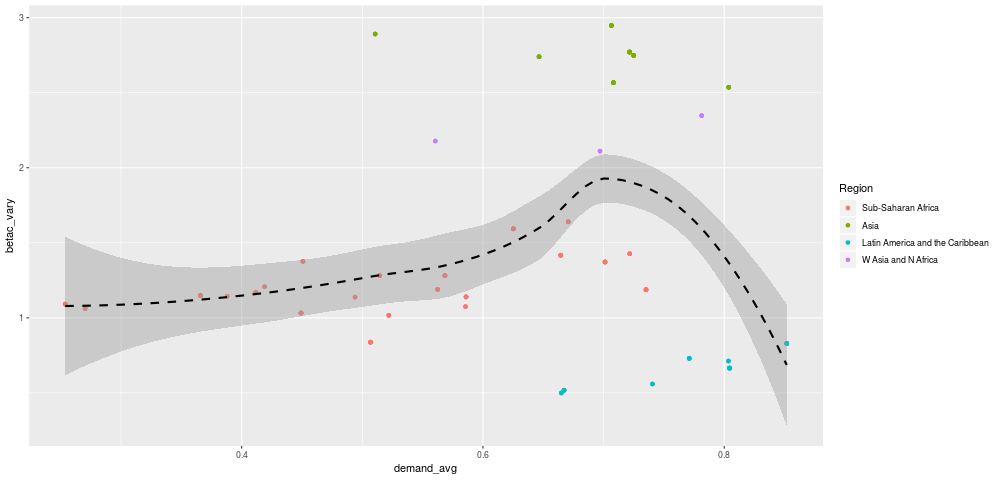
\includegraphics[scale=0.4]{2.png}
\end{center}
\newpage
 
\subsection{with correlation}
 $ y_i|\mu_{ct},\sigma_y \sim N(\mu_{ct}, \sigma_y) $ \\
 $ logit(\mu_{ct})=  \pi_{ct} + \delta_{ct} $\\
 $ \pi_{ct} = \alpha_c + \beta_c*demand_{ct} $ \\
\begin{equation*}
  \begin{pmatrix}
  	\alpha_c \\
  	\beta_c 
  \end{pmatrix}
  \sim N_2
  \begin{pmatrix}
  	\begin{pmatrix}
    	\alpha_{r1} \\
    	\alpha_{r2}
  	\end{pmatrix}
  	\begin{pmatrix}
    	\sigma^2_{c\alpha}  $\indent$  \rho_{\alpha\beta}*\sigma_{c\alpha}*\sigma_{c\beta} \\
    	\rho_{\alpha\beta}*\sigma_{c\alpha}*\sigma_{c\beta} $\indent$ \sigma^2_{c\beta}
  	\end{pmatrix} 
  \end{pmatrix} \\
\end{equation*}

\noindent
 $ \alpha_{r1}|\alpha_{w1},\sigma_{r1} \sim N(\alpha_{w1},\sigma_{r1}) $ \\
 $ \alpha_{r2}|\alpha_{w2},\sigma_{r2} \sim N(\alpha_{w2},\sigma_{r2}) $ \\
 $ \alpha_{w1} \sim N(0,100) $ \\
 $ \alpha_{w2} \sim N(0,100) $ \\

\noindent
 $ \sigma_y \sim U(0,2) $ \\
 $\sigma_{c\alpha} \sim U(0,3) $ \\
 $\sigma_{c\beta} \sim U(0,3) $\\
 $\rho_{\alpha\beta} \sim U(-.95,1)$ \\
 $ \sigma_{r1} \sim U(0,3) $\\
 $ \sigma_{r2} \sim U(0,3) $\\
\begin{center}
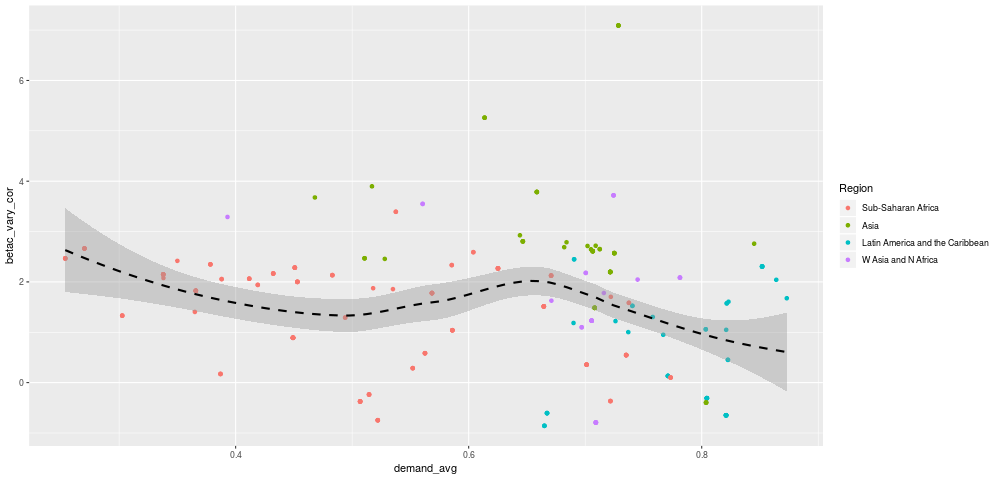
\includegraphics[scale=0.4]{3.png}
\end{center}
\newpage
\subsection{prediction plots}
\begin{center}
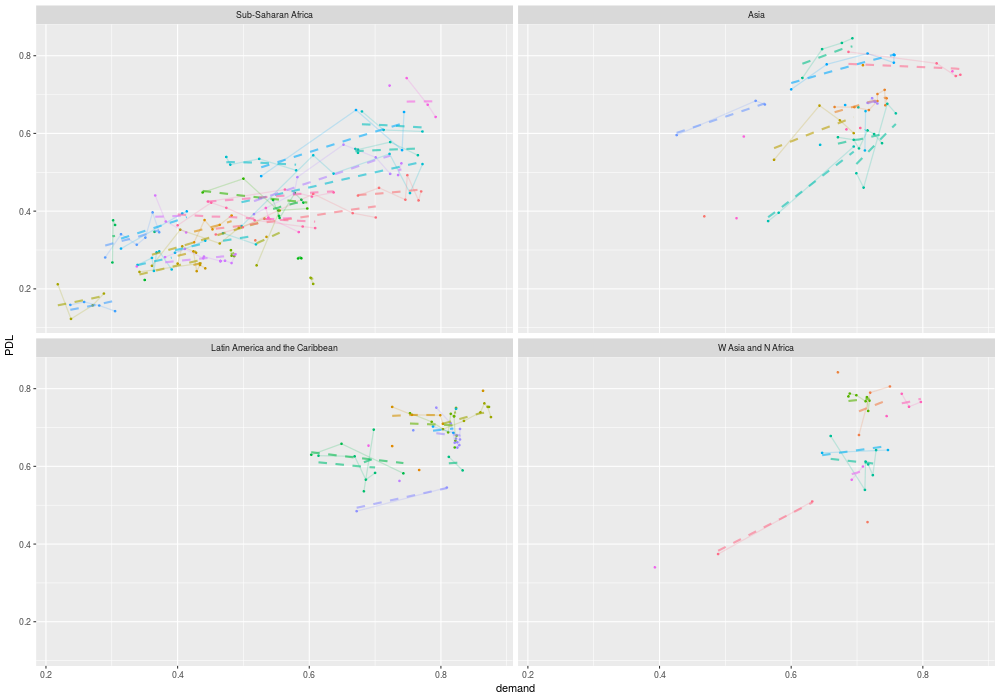
\includegraphics[scale=.5]{a.png}
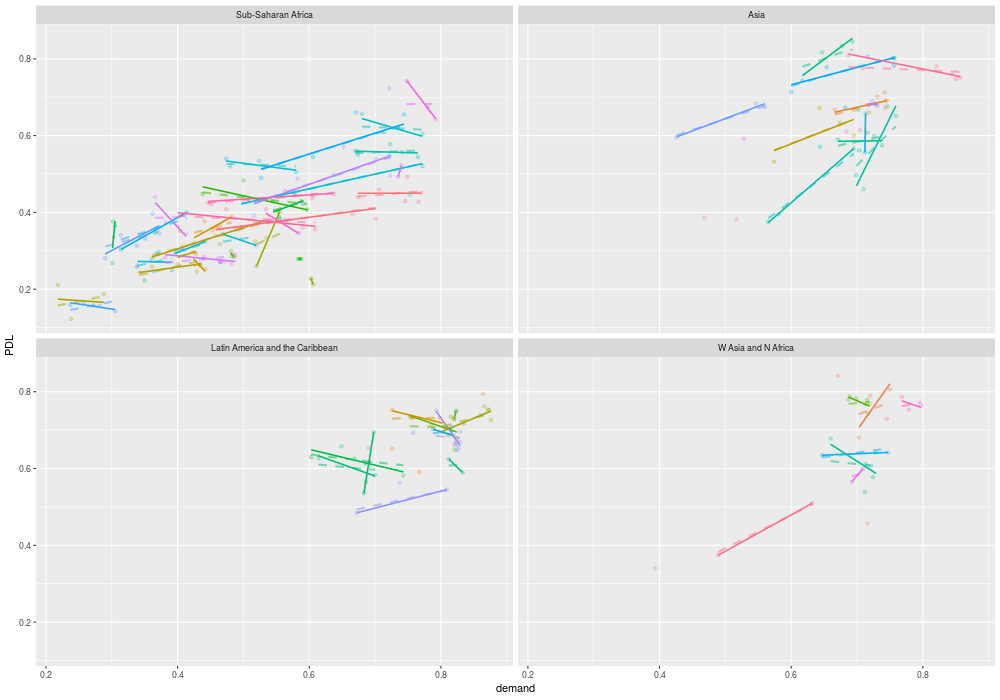
\includegraphics[scale=.5]{b.png}
\end{center}
\end{document}